\documentclass{article}

\usepackage[T1]{fontenc}
\usepackage[utf8]{inputenc}
\usepackage[polish]{babel}
\usepackage{polski}

\usepackage{lmodern}
\usepackage{amsmath}
\usepackage{graphicx}

\begin{document}
\section{Podstawowe pojęcia}
W tym rozdziale zostaną przybliżone podstawowe pojęcia związane z
geometrią obliczeniową i problemami dotyczącymi wielokątów wypukłych.

\begin{itemize}
\item{wielokąt wypukły} --- wielokąt prosty którego wnętrze jest
  zbiorem wypukłym: wszystkie punkty należące do odcinka łączącego dwa
  dowolne punkty ze zbioru wypukłego należą do tego zbioru

  \begin{figure}[htp]
    \centering
    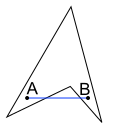
\includegraphics{img/nonconvex}
    \caption{Figura niebędąca wielokątem wypukłym.}
  \end{figure}

\item{średnica zbioru punktów} --- średnicą zbioru punktów nazywamy
  największą odległość pomiędzy dwoma punktami należącymi do zbioru

\item{lewoskrętność, prawoskrętność} --- o kącie mówimy, że jest
  lewoskrętny jeżeli wyznacznik 3 x 3 współrzędnych punktów $p_1, p_2,
  p_3$ kąta jest dodatni, w przeciwnym przypadku mówimy, że kąt jest
  prawoskrętny. Jeżeli $p_i = (x_0, y_0)$ to wyznacznik:

  \begin{center}
    \begin{math}
      \begin{vmatrix}
        x_1 & y_1 & 1 \\
        x_2 & y_2 & 1 \\
        x_3 & y_3 & 1
      \end{vmatrix}
    \end{math}
  \end{center}

\item{proste wspierające} --- prostymi wspierającymi dla wielokąta
  nazywamy takie proste, które przechodząc przez wierzchołek wielkąta
  nie przecinają jego wnętrza

\item{punkty antypodyczne} --- taka para wierzchołków wielokąta przez
  które można poprowadzić równoległe proste wspierające

\item{notacja dużego O} --- notacja asymptotycznego tempa wzrostu
  wartości funkcji względem jej argumentów, w algorytmice stosowana do
  charakterystyki złożoności obliczeniowej algorytmów opisując ilość
  potrzebnych zasobów (czasu lub pamięci) w stosunku do rozmiaru
  danych wejściowych. Mówimy, że funkcja $f$ jest co najwyżej rzędu
  $g$, gdy istnieją takie stałe $n_0 > 0$ oraz $c > 0$, że:

  \begin{center}
    $\forall n \geq n_0 : f(n) \leq c \cdot g(n)$
  \end{center}

\end{itemize}

\end{document}

%%% Local Variables:
%%% mode: latex
%%% TeX-master: t
%%% End:
